% Graphs are versatile mathematical structures that represent complex interactions and relationships between entities, providing an abstract yet intuitive representation of real-world systems. To effectively capture the rich information inherent in graph data, GNNs \cite{2016Convolutional_ChebNet,velivckovic2017gat,hamilton2017graphsage} have emerged as a transformative tool for learning from interconnected data, achieving remarkable success across a variety of domains, including database systems \cite{qgdatabase,robinson2015graph,ngdatabase,cvitkovic2020supervised}, social networks \cite{app10041327,ijcai2018p142}, recommendation systems \cite{su2024dcl, LightGCN, cai2023app_gnn_rec3}, biological networks \cite{NIPS2017_f5077839,10.1093/bioinformatics/bty294,10149537}, and more others.
Graphs are versatile mathematical structures that represent complex interactions and relationships between entities, offering an abstract yet intuitive framework for modeling real-world systems. In the context of database systems, graphs provide a powerful means to represent and analyze relational data, enabling insights into structured information. To effectively capture the rich and interconnected information inherent in graph data, GNNs \cite{2016Convolutional_ChebNet,sun2023adpa,luo2024classic} have emerged as transformative tools, achieving remarkable success in optimizing database query performance \cite{qgdatabase,robinson2015graph,ngdatabase,cvitkovic2020supervised}, enhancing data management \cite{angles2018introduction,aggarwal2010graph}, and supporting other fields such as social networks \cite{app10041327,ijcai2018p142}, recommendation systems \cite{su2024dcl, LightGCN, cai2023app_gnn_rec3}, biological networks \cite{NIPS2017_f5077839,10.1093/bioinformatics/bty294,qu2023app_gnn_bio2} and data mining \cite{ieeedataming2012,wsdmdataming2021}.

% 图数据分析与应用的重要性，gnn成为当前主流方法


Nowadays, the majority of machine learning paradigms are primarily driven by data for the acquisition of knowledge, fundamentally transforming decision-making processes across various fields \cite{wu2020gnn_survey1,zhou2022gnn_survey2,bessadok2022gnn_survey3}. However, the indiscriminate use of data has intensified the conflict between data rights and user privacy \cite{liu2020privacy,tanuwidjaja2020privacy,wu2022survey}. In response to these pressing issues, a range of pioneering regulatory frameworks has been proposed, including the European Union’s General Data Protection Regulation (GDPR) \cite{GDPR}, and the California Consumer Privacy Act (CCPA) \cite{CCPA1} in California.
% the Personal Information Protection and Electronic Documents Act (PIPEDA) \cite{PIPEDA}, and the Canadian
% Consumer Privacy Protection Act (CPPA) \cite{CCPA2}. 
Among these regulations, one of the most critical and contentious provisions is \emph{the right to be forgotten} \cite{kwak2017let}. To technically align the effectiveness of machine learning with data rights and privacy regulations, a revolutionary frontier—machine unlearning \cite{Cao2015Towards, Xu2023ACMMU} has emerged.
% 隐私保护的重要性，引出研究主题

% Despite the significant advancements in traditional machine unlearning for independently distributed data, the growing complexity of machine learning systems has underscored the rising importance of graph-structured data across various domains.
Despite advances in traditional machine unlearning for independently distributed data, the growing reliance on graph-structured data in various fields like database systems and data mining highlights the significance of GU. As graphs underpin relational schemas and mined patterns, GU enables selective removal of sensitive information while preserving the integrity of analytical results. 
% the increasing complexity of machine learning systems highlights the growing importance of graph-structured data.
% Building on this foundation, GU has emerged as a critical extension of unlearning techniques, specifically designed to meet the needs of graph-based machine learning models. 
Unlike other domains, removing specific information from a graph requires not only deleting or modifying individual nodes or edges but also needs to consider how these changes ripple through the entire graph. In addition, GU is jointly determined by downstream tasks and unlearning requests. Downstream tasks include node classification, link prediction, and graph classification (See Sec. \ref{downstream}), while unlearning requests span multiple levels, such as node, edge, and feature (See Sec. \ref{unlearning_request}). The interplay of these two aspects makes GU even more complex.
% Additionally, the combination of unlearning requests across multiple levels (i.e., node, edge, and feature) along with downstream tasks (i.e., node classification, link prediction, and graph classification) generates complex task combinations that further complicate GU (See Sec. \ref{downstream} and Sec. \ref{unlearning_request}).
% Additionally, the diversity of unlearning requests and the variety of downstream tasks further complicate GU. Different use cases may require distinct unlearning strategies, whether it's erasing sensitive information or modifying the graph for specific tasks, making GU inherently more complex and diverse than traditional machine unlearning techniques. 
These challenges position GU as a particularly demanding area of research, requiring tailored solutions for its structural complexities and task-specific needs.
% 从machine unlearning到GU 深入分析一下 graph unlearning：客观分析 gu 的复杂性（图实体错综复杂交互，难以量化 unlearning）与多样性（graph-based unlearning request and downstream tasks 存在多种类型）
Recently, a variety of GU methods has surfaced, paving the way for more responsible and privacy-compliant graph learning through data-level techniques, architectural changes, and parameter update strategies.
% . These methods address the challenge from multiple angles, such as data-level techniques, architectural modifications, and parameter update strategies. 
% 现有研究的进展（简要介绍

Though these GU strategies have made strides from various perspectives, there are still deficiencies in achieving unity: (1) \textbf{Datasets}: The utilization of different datasets (i.e., domain and scale) and rigidity of processing data regarding splitting and inference settings make it difficult to analyze the results. 
(2) \textbf{Backbones}: The lack of harmonization among GNN backbones between different methods creates barriers for fair comparisons. (3) \textbf{Experiments}: Typically, experiments are conducted on a single downstream task under one type of unlearning request, which prevents cross-examining of downstream tasks under different unlearning requests. Besides, the varying configurations of unlearning requests and differing evaluation metrics in existing methods lead to divergent interpretations in experimental results. These challenges highlight the urgent need for a standardized benchmark to establish a unified and comprehensive understanding of the GU landscape.
% 当前领域的研究困境（我们提出这一领域 benchmark 的主要动机）：没有统一的测试基准，阻碍了当前领域发展等等，然后说我们这个 benchmark 有助于研究者们推动这一领域的发展（除了开发benchmark的通用优点，我们最好结合gu说一些额外的优势 == 比如因为 unlearning request 和下游任务的多样性，benchmark可以提供全面的评估环境等等）

To address the aforementioned challenges, we propose OpenGU in this paper, to the best of our knowledge, the first comprehensive benchmark specifically designed for graph unlearning. OpenGU integrates $16$ recently proposed SOTA algorithms and $37$ multi-domain datasets, enabling the flexible $3\times3$ combination of unlearning requests and downstream tasks. OpenGU implements these components with unified APIs to address three types of unlearning requests. Based on this design, we conduct an in-depth investigation of these GU algorithms, offering valuable insights in terms of three dimensions: effectiveness, efficiency, and robustness. For \textbf{effectiveness}, OpenGU provides a comprehensive evaluation in two aspects: model updating and inference protection. We fairly assess the forgetting ability for unlearning entities and the reasoning capability for retained data to determine whether the methods achieve effective trade-off between forgetting and reasoning. For \textbf{efficiency}, OpenGU provides insights into scalability by evaluating how well GU methods can handle increasing amounts of data and more complex graph structures, showing their practical applicability in real-world scenarios. Furthermore, we analyze the computational resources required by various graph unlearning algorithms, focusing on time and space complexity from both theoretical and empirical perspectives. For \textbf{robustness}, we focus on noise and sparsity scenarios in real-world applications, and delve into the algorithms' capacity to maintain performance stability and integrity amid different unlearning intensities. 
% 我们的 opengu 都有啥（客观阐述框架内容）


\textbf{Our contributions}. We propose OpenGU, the inaugural benchmark specifically tailored for GU domain. Our contributions are outlined as follows:
% \begin{itemize}[leftmargin=*,noitemsep,topsep=0pt,parsep=0pt]
    % \item 
(1) \underline{\textit{Comprehensive Benchmark.}} OpenGU integrates $16$ SOTA algorithms and $37$ popular multi-domain datasets, establishing a thorough evaluation framework for a fair comparison. Moreover, OpenGU expands and standardizes experimental task requirements, encompassing unlearning requests and downstream tasks, thereby facilitating a code-level implementation of $3\times3$ cross-experiment configurations.
(2) \underline{\textit{Analytical Insights.}} Through extensive empirical experiments centered around algorithms' forgetting capability and reasoning capability, we conduct a thorough analysis 
% from the perspectives of effectiveness, efficiency and robustness, 
and summarize $8$ key conclusions, envisioning our conclusions as the catalyst for GU field. 
(3) \underline{\textit{Open-sourced Benchmark Library.}} OpenGU is designed as an open-source benchmark library, providing researchers and practitioners with accessible tools and resources for expanding the exploration of GU. Additionally, comprehensive documentation and user-friendly interfaces foster collaboration and innovation within the GU community. Our code is available at \href{https://github.com/bwfan-bit/OpenGU}{https://github.com/bwfan-bit/OpenGU}.
% （8）第八部分：our contribution（推销一下 openfgl 的写法，不要list而是斜体下划线，我感觉更好看）
% **注意一下，不一定每一部分占据一段，这个是我简单梳理的一个逻辑关系，可以在写的过程不断完善，有遗漏或者逻辑不通顺的地方我们也可以随时讨论
% \end{itemize}

\captionsetup[figure]{}
\begin{figure*}[h]
  \centering
  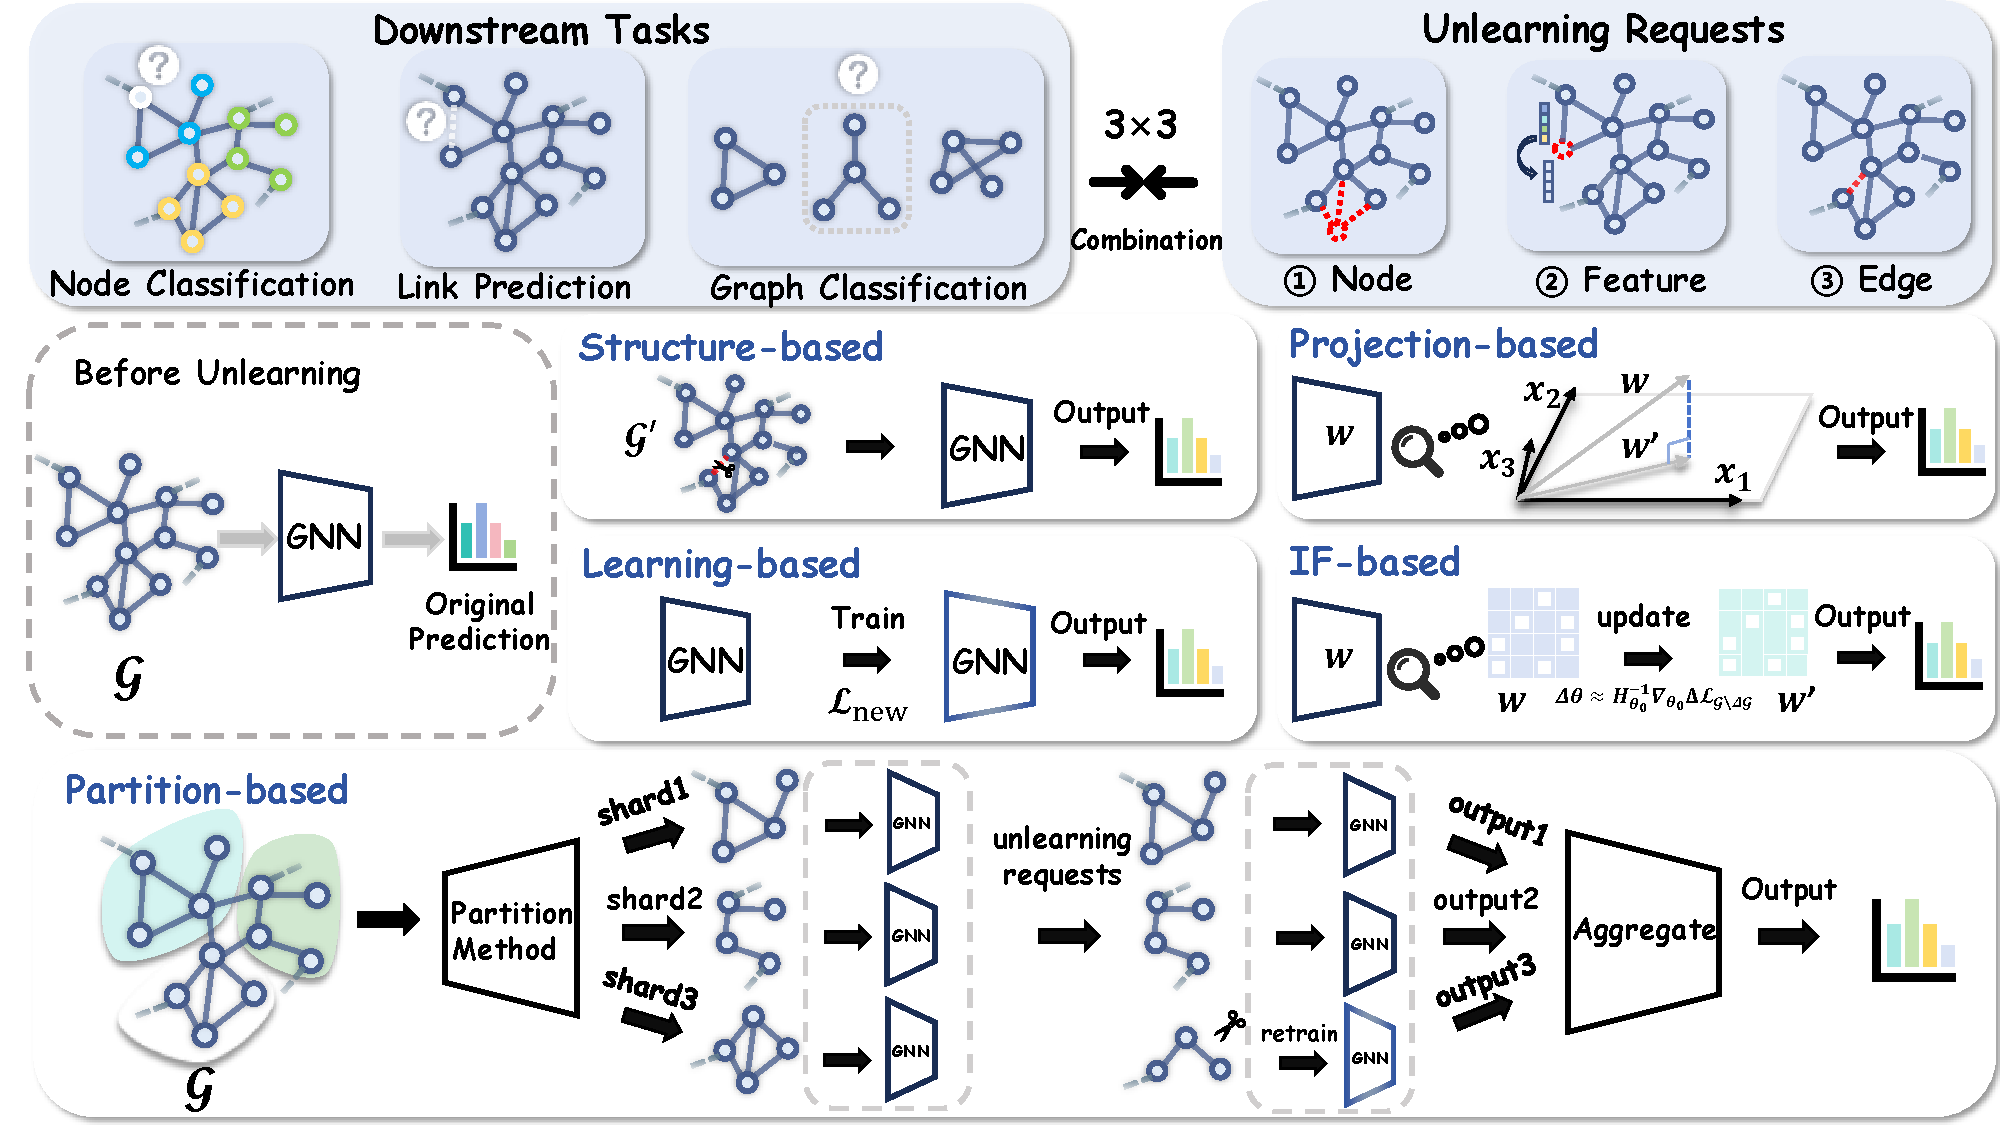
\includegraphics[width=1\linewidth,height=0.55\linewidth]{Pic/OpenGU.pdf}
  \caption{An overview of the OpenGU framework, illustrating the key components and methodologies involved in GU.}
  \vspace{-0.3cm}
  \label{figure1}
\end{figure*}


